\chapter{Neexpandující impulzní gravitační vlny}
Neexpandující impulzní vlny 


\section{Konstrukce}
Nejprve popíšeme několik způsobů konstrukce prostoročasů s neexpandujícíme impulzními gravitačními vlnami, začneme Penroseovou \cite{Penrose:1972xrn} geometrickou metodou
"cut and paste" a zavedeme spojité souřadnice na tomto prostoročase. Dále zavedeme distribuční popis těchto prostoročasů

\subsection{"Cut and paste"\ metoda konstrukce}
\label{sec:cut_and_paste_konstrukce1}
Geometrická metoda konstrukce "cut and paste" impulzních gravitačních vln v Minkowského prostoročase \eqref{eq:minkowski} se zakládá na rozdělení celého prostoročasu podél rovinné
světelné nadplochy $\mathcal{N}$ kde je implulzní vlna lokalizována na dvě části $\mathcal{M}^+$ a $\mathcal{M}^-$. Opětovným spojením těchto částí a ztotožněním bodů na hranici
řezu $\mathcal{N}$ se specifickým posunutím dostaneme prostoročas s impulzní gravitační vlnou.

\begin{figure}[h]\centering
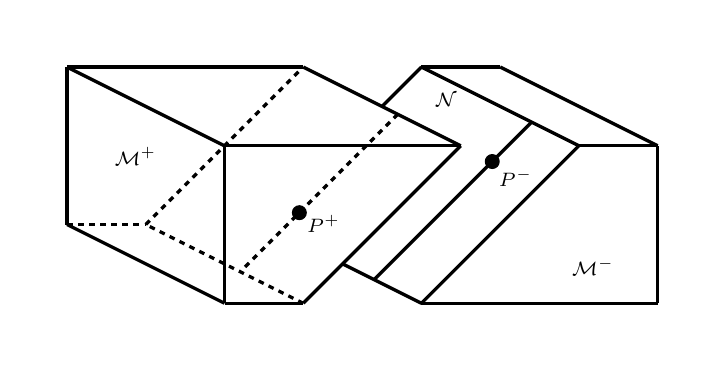
\begin{tikzpicture}
\clip(-2.5,-0.5) rectangle (6.,3.5);
\draw [line width=1.2pt] (-2.,1.)-- (0.,0.);
\draw [line width=1.2pt] (-2.,3.)-- (-2.,1.);
\draw [line width=1.2pt] (0.,0.)-- (0.,2.);
\draw [line width=1.2pt] (0.,2.)-- (-2.,3.);
\draw [line width=1.2pt] (-2.,3.)-- (1.,3.);
\draw [line width=1.2pt] (0.,2.)-- (3.,2.);
\draw [line width=1.2pt] (1.,3.)-- (3.,2.);
\draw [line width=1.2pt] (0.,0.)-- (1.,0.);
\draw [line width=1.2pt] (1.,0.)-- (3.,2.);
\draw [line width=1.2pt,dash pattern=on 2pt off 2pt] (1.,0.)-- (-1.,1.);
\draw [line width=1.2pt,dash pattern=on 2pt off 2pt] (-2.,1.)-- (-1.,1.);
\draw [line width=1.2pt,dash pattern=on 2pt off 2pt] (-1.,1.)-- (1.,3.);
\draw [line width=1.2pt] (2.5,0.)-- (4.5,2.);
\draw [line width=1.2pt] (2.5,0.)-- (5.5,0.);
\draw [line width=1.2pt] (5.5,0.)-- (5.5,2.);
\draw [line width=1.2pt] (4.5,2.)-- (5.5,2.);
\draw [line width=1.2pt] (4.5,2.)-- (2.5,3.);
\draw [line width=1.2pt] (5.5,2.)-- (3.5,3.);
\draw [line width=1.2pt] (2.5,3.)-- (3.5,3.);
\draw [line width=1.2pt] (2.,2.5)-- (2.5,3.);
\draw [line width=1.2pt] (2.5,0.)-- (1.5,0.5);
\draw [line width=1.2pt] (1.9,0.3)-- (3.9,2.3);
\draw [line width=1.2pt,dash pattern=on 2pt off 2pt] (2.2,2.4)-- (0.2,0.4);
\begin{scriptsize}
\draw[color=black] (-1.1302677200189184,1.864045432930641) node {$\mathcal{M}^+$};
\draw[color=black] (2.8186222701156605,2.585603404549911) node {$\mathcal{N}$};
\draw[color=black] (4.6815537604781525,0.46028719723496975) node {$\mathcal{M}^-$};
\draw [fill=black] (0.9503176308657735,1.1503176308657732) circle (2.5pt);
\draw[color=black] (1.2574332042485015,1.0112951028351398) node {$P^+$};
\draw [fill=black] (3.4,1.8) circle (2.5pt);
\draw[color=black] (3.6976110719064135,1.5885414801305562) node {$P^-$};
\end{scriptsize}
\end{tikzpicture}
\caption{Geometrická konstrukce neexpandující impulzní gravitační vlny pomocí metody "cut and paste", 
podél nadplochy $\mathcal{N}$ dojde k rozdělení prostoročasu na dvě části $\mathcal{M}^+$ a $\mathcal{M}^-$ 
a opětovnému ztotožnění bodů na hranici obou částí se specifickým posunem.}
\label{obr01:geomkonstrukt}
\end{figure}

Pro světelnou nadplochu $\mathcal{N}$ danou podmínkou $\mathcal{U}=0$ pak tato konstrukce odpovídá Penroseově 
spojovacím podmínkám

\begin{equation}
    \label{eq:lepici_podminky}
\left[\eta, \bar{\eta}, \mathcal{V}, \mathcal{U}=0_- \right]_{\mathcal{M}^-} \equiv 
\left[\eta, \bar{\eta}, \mathcal{V}-H\left(\eta, \bar{\eta}\right), \mathcal{U}=0_+  \right]_{\mathcal{M}^+},
\end{equation}
kde $H(\eta, \bar{\eta})$ je holomorfní. Penrose \cite{Penrose:1972xrn} ukázal, že impulzní gravitační vlny
jsou v tenzoru křivosti reprezentovány členy proporciálními Diracově delta distribuci $\delta(\mathcal{U})$.
V Minkowského pozadí je nadplocha $\mathcal{U}=0$ rovina a řešení spadá do rodiny impulzních $pp-$vln, tedy
rovnoběžně se propagujících rovinných vln. Obecně na pozadích konstantní křivosti platí stejné napojovací podmínky
\eqref{eq:lepici_podminky} a nadplocha představuje $\mathcal{U}=0$ plochu konstantní Gaussovské křivosti 
$K=\frac{1}{3}\Lambda$ která je popsána metrikou $d\sigma^2=2(1+\frac{1}{6}\Lambda \eta \bar{\eta})^{-2} 
d\eta~d\bar{\eta}$. V případě $\Lambda \neq 0$ se tedy jedná buďto o sféru
($\Lambda > 0$) nebo o hyperboloid ($\Lambda < 0$). Popis těchto nadploch konstatní křivostsi v (A)dS prostoročasech a
jejich geometrické vlastnosti jsou shrnuty v \cite{Podolsky:1997ri}, kde je také ukázáno,
že se jedná o neexpandující nadplochy.

%%%TODO Cut and paste pro \Lambda \neq 0 - obrázek hyperboloidu

\subsection{Spojitý tvar metriky}
Metoda "cut and paste"\ nám dává identifikaci bodů prostoročasu na obou stranách impulzní vlny a tedy napojovací podmínky
pro geodetiky, nic ale neříká o podobě metriky kompletního prostoročasu s impulzní vlnou. Potřebujeme tedy najít vhodný
souřadnicový systém, ve kterém bude metrika spojitá funkce $\mathcal{U}$. Toho dosáhneme postupem použitým např. v
\cite{Podolsky:2014ysa}, kde z metriky prostoročasu pozadí \eqref{eq:konfmetric}, respektive
\begin{equation}
    \label{eq:null_background_metric}
    \mathrm{d}s_0^2 = \frac{2~\mathrm{d}\eta~\mathrm{d}\bar{\eta}-2~\mathrm{d}\mathcal{U}~\mathrm{d}\mathcal{V}}
    {\left[1+\frac{1}{6}\Lambda \left(\eta \bar{\eta}
    -\mathcal{U}\mathcal{V}\right)\right]^2},
\end{equation}
souřadnicovou transformací
\begin{equation}
    \label{eq:nonexp_cont_transform}
    \mathcal{U}=U,~~~~ \mathcal{V}=V+H+UH_{,Z}H_{,\bar{Z}},~~~~ \eta=Z+UH_{,\bar{Z}},
\end{equation}
kde uvažujeme libovolnou reálnou funkci $H(Z, \bar{Z})$, obdržíme metriku
\begin{equation}
    \label{eq:nonexp_cont_nokink_metric}
    \mathrm{d} s^{2}=\frac{2\left|\mathrm{d} Z+U\left(H_{, Z \bar{Z}} 
    \mathrm{d} Z+H_{, \bar{Z} \bar{Z}} \mathrm{d} \bar{Z}\right)\right|^{2}-2 \mathrm{d} U 
    \mathrm{d} V}{\left[1+\frac{1}{6} \Lambda(Z \bar{Z}-U V-U G)\right]^{2}}
\end{equation}
kde $G(Z, \bar{Z}) \equiv H - Z H_{,Z}-\bar{Z}H_{,\bar{Z}}$. Metriku \eqref{eq:nonexp_cont_nokink_metric} pak 
uvažujeme pouze pro $U>0$, zatímco na $U<0$ uvažujeme metriku \eqref{eq:null_background_metric}. Definováním
tzv. kink funkce jako
\begin{equation}
    \label{eq:kink_function}
    U_+ \equiv U_+(U) = \begin{cases}
        0 & \text{pro } U \leq 0 \\
        U & \text{pro } U \geq 0
    \end{cases}
\end{equation}
můžeme výslednou metriku zapsat jako
\begin{equation}
    \label{eq:nonexp_continuous_metric}
    \mathrm{d} s^{2}=\frac{2\left|\mathrm{d} Z+U_+\left(H_{, Z \bar{Z}} 
    \mathrm{d} Z+H_{, \bar{Z} \bar{Z}} \mathrm{d} \bar{Z}\right)\right|^{2}-2 \mathrm{d} U 
    \mathrm{d} V}{\left[1+\frac{1}{6} \Lambda(Z \bar{Z}-U V-U_+ G)\right]^{2}}.
\end{equation}
Transformaci \eqref{eq:nonexp_cont_transform} lze pomocí Heavisideovy funkce $\Theta(U)$ přepsat do tvaru
spojujícího metriku \eqref{eq:null_background_metric} s metrikou \eqref{eq:nonexp_continuous_metric}
\begin{equation}
    \label{eq:nonexp_cont_full_transform}
    \mathcal{U}=U,~~~~ \mathcal{V}=V+\Theta(U) H + U_+ H_{,Z}H_{,\bar{Z}},~~~~ \eta=Z+ U_+ H_{,\bar{Z}}.
\end{equation}
Tato transformace obsahuje Penroseovy spojovací podmínky \eqref{eq:lepici_podminky} v $U=0$, kde
vzniká nespojitost v souřadnici $\mathcal{V}$. Tato metoda konstrukce tedy představuje explicitní "cut and paste"\ konstrukci.



\subsection{Distribuční tvar metriky}
Dalším způsobem konstrukce impulzní gravitační vlny je limitní přechod od příslušných rodin tzv. "sandwichových"\
gravtiačních vln s hladkým profilem vlnoplochy k limitnímu distribučnímu vyjádření impulzní vlny. Takové vyjádření
také dostaneme dosazením invezní transformace k \eqref{eq:nonexp_cont_full_transform} do spojité metriky 
\eqref{eq:nonexp_continuous_metric}.

\begin{equation} \label{eq:nonexp_distr_metric_omega}
\mathrm{d}s^2=\frac{2\mathrm{d}\eta~\mathrm{d}\bar{\eta} - 2 \mathrm{d}\mathcal{U}~\mathrm{d}\mathcal{V} + 2H(\eta, \bar{\eta}) \delta(\mathcal{U}) 
~\mathrm{d}\mathcal{U}^2}{\left[1+\frac{1}{6}\Lambda(\eta \bar{\eta}-\mathcal{U}\mathcal{V})\right]^2}
\end{equation}

\subsection{Boost Schwarzchildova řešení}
%%% TODO nechat to tady???
Další způsob, kterým lze prostoročas s impulzní pp-vlnou získat je boost Schwarzchildova řešení

\section{Interakce s testovacími částicemi}

\subsection{Profil impulsní gravitační vlny}

Einsteinovy rovnice \eqref{eq:einsten_field_equations} se pro metriku \eqref{eq:nonexp_distr_metric_omega}
redukují na 

\subsection{Refrakční rovnice}
\textcolor{red}{Zde více komentáře (ex. souř. systém kde jsou geodetiky spojité,
zavést C1 matching a ospravedlnit použití refrakčních rovnic)}
Změna polohy (nalepení geodetiky) je dána Penroseovými spojovacími podmínkami, tento skok ale generuje změnu v derivacích poloh a dojde tedy
k refrakci geodetik na impulzní nadploše $\mathcal{U}=0$ podle sady tzv. refrakčních rovnic
\begin{align}
    \label{eq:refraction_nonexpanding}
    \begin{split}
        &\dot{\mathcal{U}}^{+}_{\mathrm{i}} = \dot{\mathcal{U}}^{-}_{\mathrm{i}}\\
        &\dot{\mathcal{V}}^{+}_{\mathrm{i}} = \dot{\mathcal{V}}_{\mathrm{i}}^{-} + H_{\mathrm{i}, Z}
        \dot{\eta}^{-}_{\mathrm{i}} + H_{\mathrm{i}, \bar{Z}} \dot{\overline{\eta}}^{-}_{\mathrm{i}} + 
        H_{\mathrm{i}, Z} H_{\mathrm{i}, \bar{Z}} \dot{\mathcal{U}}_{\mathrm{i}}^{-}\\
        &\dot{\eta}_{\mathrm{i}}^{+} =\dot{\eta}_{\mathrm{i}}^{-}+H_{\mathrm{i}, \bar{Z}}
        \dot{\mathcal{U}}_{\mathrm{i}}^{-}.
    \end{split}
\end{align}
Index $i$ znamená hodnotu na impulzní nadploše, složky označené znakem + jsou za impulzem a tedy v části prostoročasu $\mathcal{M}^+$,
složky označené znakem - jsou před impulzem v $\mathcal{M}^-$.
%%%TODO 5D formalismus pro konformně ploché pč


\subsection{Interakce}
\textcolor{red}{Zde vykreslené obrázky s popisem, jak pro světelné částice tak pro
časupodobné geodetiky (případně i pro srandu prosoturupodobné)}
